\documentclass[a4paper,12pt]{article}
\usepackage[top = 3cm, bottom = 2cm, left = 3cm, right=2cm]{geometry}
\usepackage[utf8]{inputenc}
\usepackage{amsmath,amsfonts,amssymb}
\usepackage{float}
\usepackage{graphicx}
\usepackage[english]{babel}
\usepackage{indentfirst}
\usepackage{float}
\usepackage{textcomp}
\usepackage{gensymb}
\usepackage{subfigure}
\usepackage{enumerate}
\title{CDM Description - ARAM}

\begin{document}
	\maketitle
	\section{CDM Development}
	Knowing that the aparent solar diameter observed on the celestial vault is aproximately $0,5^{\circ}$, it was assumed, for each cylinder of sensor element, the value of $2^{\circ}$ as  FoV, Fiel of View. This value represents a detection region that covers 4 solar diameters. 
	
	The figure 1 represents the initial cylinder that comports a LDR. The calculations below were based on Figure 1. Remembering that R: LDR radius and L: the cylinder length.

\begin{figure}[htb] 
	\centering
	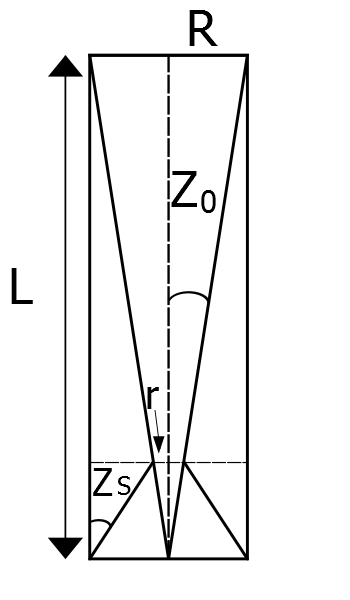
\includegraphics[scale=0.5]{MCD_1.jpg}
	\caption{First version of a cylinder to the sensors matrix.}
\end{figure}

$$\frac{R}{L} = tan(Z_{0}) ; \,\,   R = \frac{D_{LDR}}{2}, Z_{0} = \frac{FoV}{2}$$
$$L = \frac{R}{tan(Z_{0})} \longrightarrow L = \frac{2}{tan(1^{o})}  \longrightarrow L \cong 115 mm$$ 

\newpage
It was found that the length of the tube was too large relative to its diameter, this causes a problem in quality of the printed resistant plastic, therefore it was necessary to add the parameter $Z_{0}$ to the tube. This parameter not only changed the geometry of the cylinder into a conical trunk, but also enabled the preservation of the FoV of each cylinder as well as the reduce its length by approximately 50\% ,features that facilitate the 3D prototyping process and guarantee proportionality in the CDM dimensions.
	

$$Tan(Z_{s}) = \frac{(R-r)}{L_{novo}}  \, ; \,  onde: \, r= \,1mm \,e \, L_{novo}= \, 60mm $$
$$Tan(Z_{s}) = \frac{(2-1)}{60}  \longrightarrow   Z_{s} = Tan^{-1}(0,0167) \therefore Z_{s} \cong 1^{\circ} $$

Once dimensioned each cylinder, another problem was found: having more than one sensor tracking the sun in the same time. This problem happens because the sun is located to millions of kilometers away from land, and in the first version of the matrix of sensors, the axes of the tubes were dimensioned parallel to each other, in other words, the cylinders point to the same region. The solution developed to correct this problem it was to create an angular difference between the axes, tilt them.

Ensure the slope of pipes on a flat surface became quite complex, so it was  developed the CDM (Detection of Circular Matrix).

aaaaa

A fim de sanar esta problemática desenvolveu-se a MCD(Matriz Circular Detectora), composta por 25 tubos  dispostos em círculos concêntricos na superfície de uma calota esférica. Os parâmetros calculados abaixo dizem respeito ao raio da seção transversal(X), distância do centro da esfera suporte(teórica) até o início da MCD (d), o tamanho de flecha (F) e o FoV sólido da matriz(FoV$_{S}$).
\begin{figure}[htb] 
	\centering
	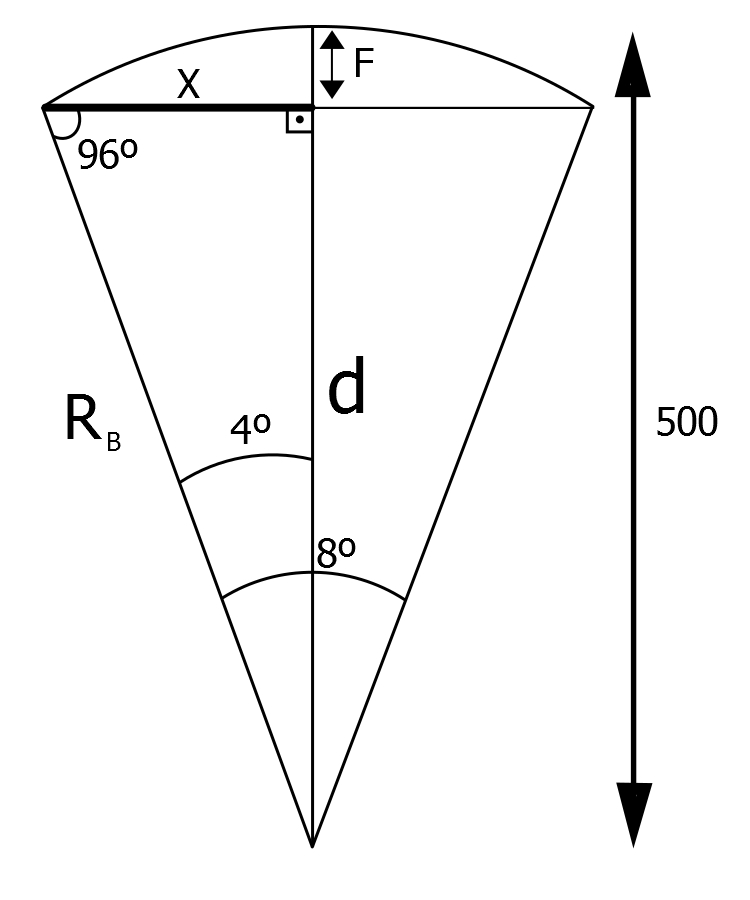
\includegraphics[scale=0.3]{MCD_2.jpg}
	\caption{MCD.}
\end{figure}
$$ \frac{X}{sin(4^{\circ})} = \frac{R_{B}}{sin(90^{\circ})}\longrightarrow X= \frac{R_{B}\times sin(4^{\circ})}{sin(90^{\circ})} \longrightarrow X=\frac{500\times 0,06975}{1} \therefore X=34,87mm $$
$$d = \sqrt{500^{2} - 34,87^{2}} \therefore d=498,78mm \, ;\, F=500-498,78 \therefore F=1,22mm $$
$$ A_{\bot } = \pi\times(34.87)^{2} \therefore A_{\bot } = 3.819,92mm^{2} $$ 
$$ FOV_{S} = \frac{A_{\bot }}{(R_{B})^{2}} \longrightarrow FoV_{S} =\frac{3.819,92}{500^{2}} \therefore FOV_{S} = 0,0153 \, strad$$ 
\newpage
Posteriormente calculou-se a distância entre cada camada de tubos da MCD, medida entre centros (S), na condição do apontamento indicado por um único tubo. 
\begin{figure}[htb] 
	\centering
	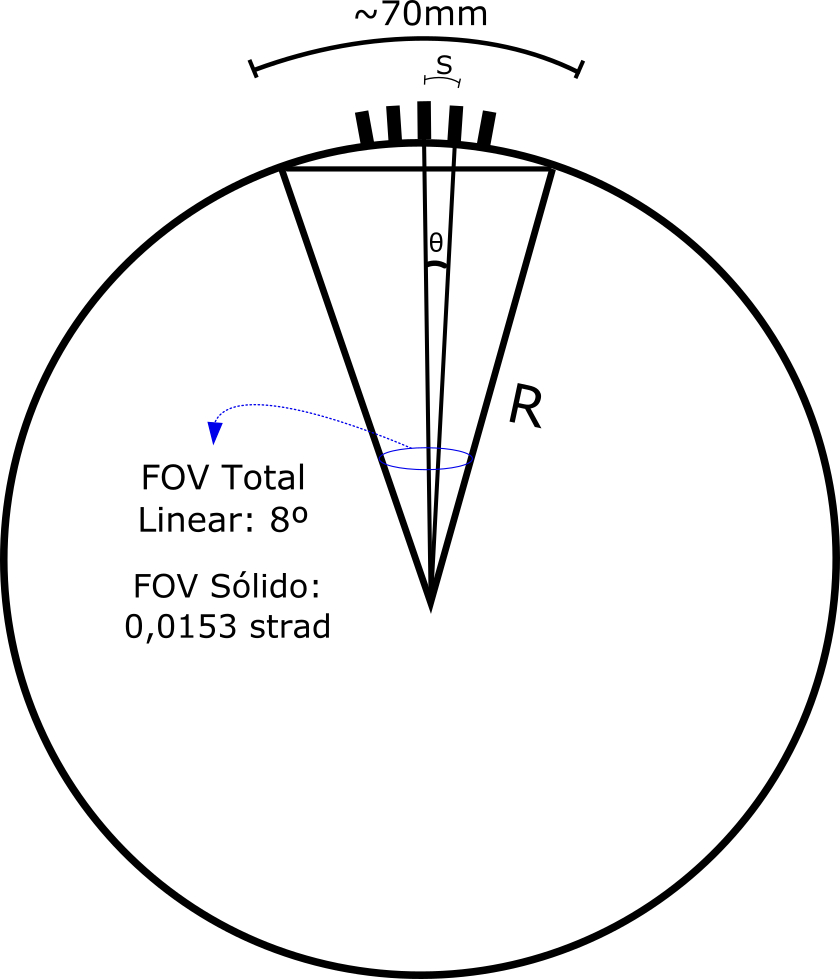
\includegraphics[scale=0.4]{MCD_3.jpg}
	\caption{MCD corte lateral.}
\end{figure}

$$ \pi \longleftrightarrow 180^{\circ}$$
$$ X_{S} \longleftrightarrow 1^{\circ}$$
$$X_{S} = \frac{\pi}{180^{\circ}} \therefore X_{S} = 0,01745\, strad$$
$$\therefore \theta = 1^{\circ} = 0,01745 \,strad$$
$$S= R\times \theta \longleftrightarrow S= 500\times 0,01745 \therefore S=8,7mm $$

Por fim, desenvolveu-se o modelo da MCD no software Creo Parametric. Nesta etapa a geometria de cada elemento colimador voltou a ser de tubo, porém, para garantir a mesma funcionalidade e FoV, cada tubo apresenta um orifício de 1mm.   As figuras 4.a, 4.b e 4.c representam o modelo desenvolvido.

\begin{figure}[h]
	
	\center
	\subfigure[ref1][Vista superior.]{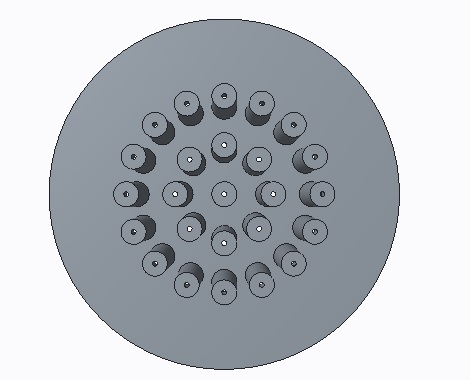
\includegraphics[width=4cm]{MCD_vista_de_cima.jpg}}
	\qquad
	\subfigure[ref2][Vista lateral esquerda.]{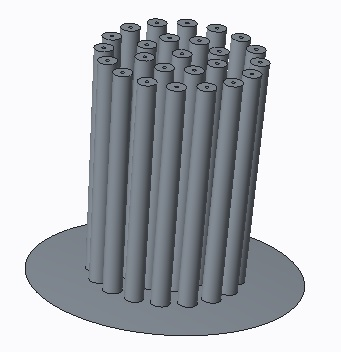
\includegraphics[width=4cm]{MCD_Lateral_esquerda.jpg}}
	\qquad
	\subfigure[ref2][Vista inferior.]{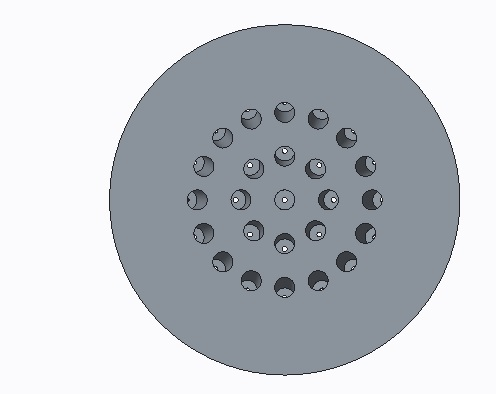
\includegraphics[width=4cm]{MCD_vista_de_baixo.jpg}}
	\caption{MCD - modelo no Creo Parametric.}
	
\end{figure}
 \section{Algoritmo de apontamento fino}

Após realizar o apontamento grosso, por efemérides, um dos sensores da MCD detecta o sol. Em seguida o algoritmo de apontamento fino calcula a distância entre o sensor que encontrou o sol e o sensor central da MCD. Com auxílio do par de motores ortogonais, o algoritmo de detecção guia o apontamento sol para o sensor que se encontra no centro da matriz de sensores.

 O sensor central foi projetado para estar alinhado com o radiômetro em escala reduzida. Pode-se dizer que este algoritmo de apontamento fino faz com que o instrumento esteja apontando efetivamente para o sol, conduzindo  o eixo principal do instrumento até a posição aonde estava o eixo do cilindro que detectou o sol. As figuras abaixo ilustram o procedimento.
 \begin{figure}[h]
 	
 	\center
 	\subfigure[ref1][Comportamento antes do apontamento grosso.]{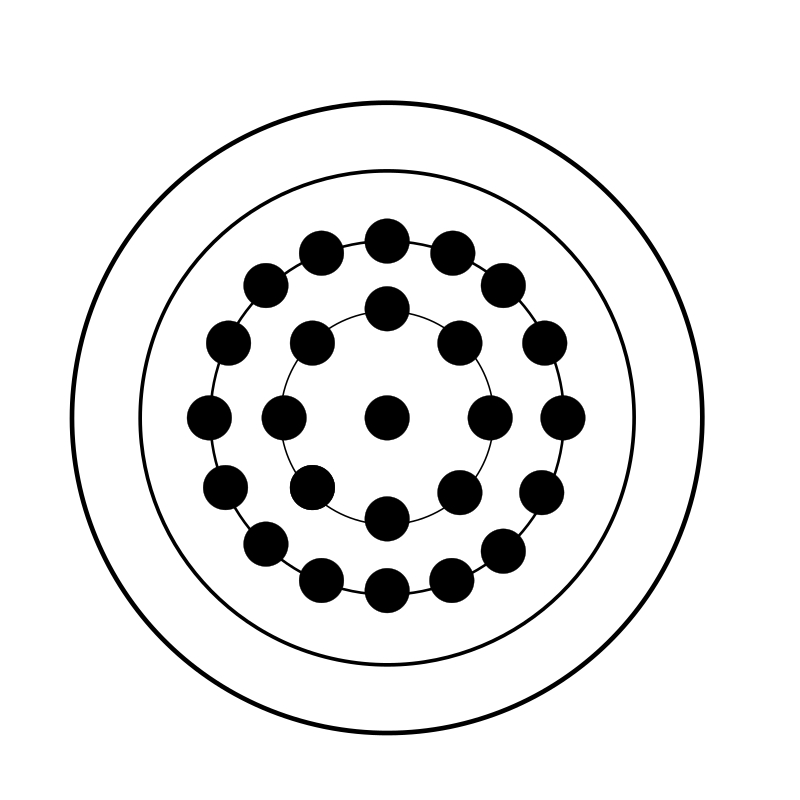
\includegraphics[width=4cm]{MCD_4.jpg}}
 	\qquad
 	\subfigure[ref2][Comportamento após o apontamento grosso.]{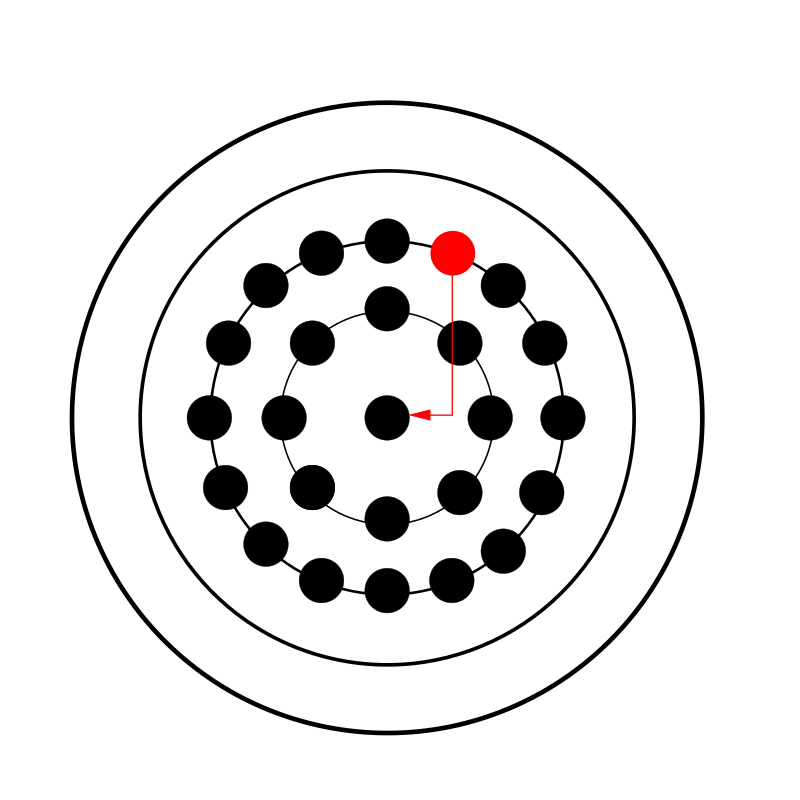
\includegraphics[width=4cm]{MCD_5.jpg}}
 	\qquad
 	\subfigure[ref2][Comportamento após apontamento fino.]{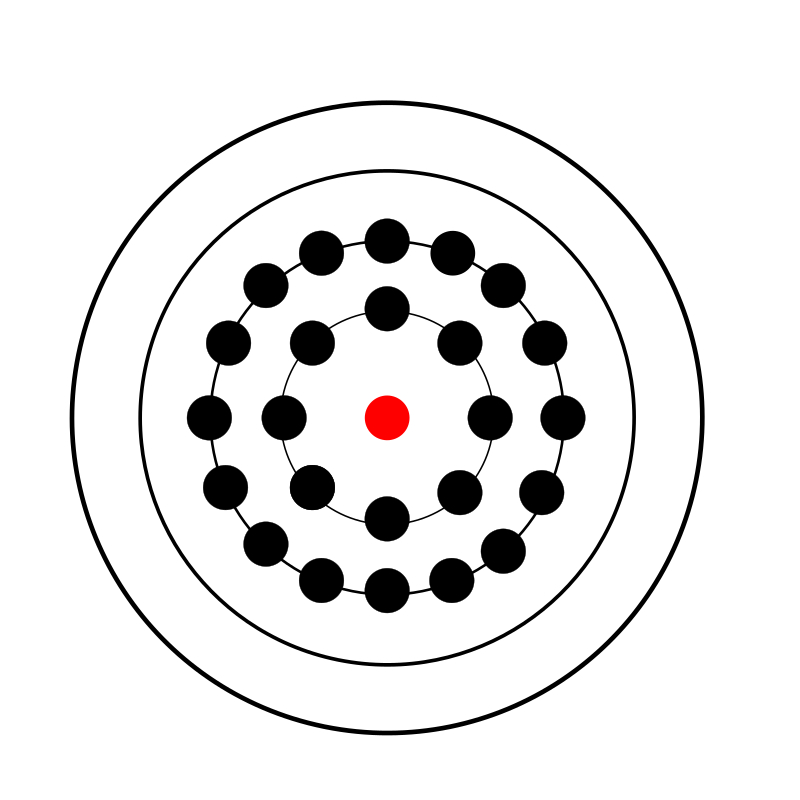
\includegraphics[width=4cm]{MCD_6.jpg}}
 	\caption{Etapas do algoritmo de apontamento fino.}
 	
 \end{figure}

\end{document}